\textbf{Beispiel 3} \\ \\
a)\\ \\
Das physikalische Prinzip, welches die Wärmeübertragung bestimmt heißt erzwungene Konvektion. Hierbei handelt es sich um eine Randbedingung dritter Art, also eine gemischte Randbedingung. \\ \\ 
b) \\ \\
Das RC-Ersatzbild sieht wie folgt aus
\begin{figure}[h]
	\centering
	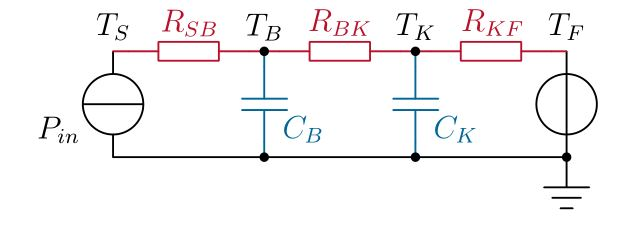
\includegraphics[width=10cm]{tikz/05_02_2016_3b}
\end{figure}
\newline
Die einzelnen Größen werden zu
\begin{align*}
	P_{in} &= I_a(U_e - U_a) \\
	R_{SB} &= aus dem Datenblatt \\
	C_B &= m_Bc_B \\
	R_{BK} &= \frac{h_p}{\lambda_p A_p} \\
	C_K = m_Kc_K &= \rho_K l_K b_k h_K c_K
\end{align*}
\newpage
\noindent
c) \\ \\ 
Ausgangspunkt sind die zur Ersatzschaltung zugehörigen Knoten- und Maschengleichungen
\begin{align*}
	sC_BT_B &= \dot{Q}_{SB} - \dot{Q}_P \\
	sC_KT_K &= \dot{Q}_P - \dot{Q}_{KF} \\
	R_{KF}\dot{Q}_{KF} &= T_K - T_F \\
	\dot{Q}_PR_{BK} &= T_B - T_K \\
	\dot{Q}_{SB}R_{SB} &= T_S - T_B \\
	\dot{Q}_{SB} &= P_{in}
\end{align*}
Löst man dieses Gleichungssystem nach $\dot{Q}_P$ erhält man
\[
	\dot{Q}_P = \frac{(C_KR_{KF}s + 1)P_{in} - C_BT_Fs}{(C_BC_KR_{BK}R_{KF}s^2 + (C_BR_{BK} + C_BR_{KF} + C_KR_{KF}) + 1)}
\]
Im stationären Fall gilt
\[
	\dot{Q}_P = P_{in}
\]
d) \\ \\
Aus der stationären Lösung aus Punkt c) folgt
\[
	P_{in} = \frac{T_S - T_F}{R_{SB} + R_{BK} + R_{KF}}
\]
somit darf der gefragte Widerstand nicht den Wert
\[
	R_{KF,max} \leq \frac{T_{S,max} - T_F}{P_{in}} - R_{SB} -R_{BK}
\]
nicht überschreiten, damit die Temperatur $T_{S,max}$ stationär nicht überschreitet.